\chapter{Sequenzdiagramm}

Im Folgenden wird der Vorgang eines vollständigen Buchungsdurchgangs betrachtet, um final mittels Sequenzdiagrammen das Vorgehen visuell darzustellen.

Bei der Erarbeitung wird aufgrund des Umfangs ein Teil der Detailtiefe entfernt. Die exakte Kommunikation mit der Datenbasis (in Realität mit einer Datenbank und im Projekt mit den CSV-Dateien) wird nicht betrachtet. Bei der Interaktion mit der Anwendung wird die Unterteilung in verschiedene GUIs unter dem Begriff 'Benutzeroberfläche' zusammengefasst. Es wird ebenfalls davon ausgegangen, dass für den Sequenzablauf benötigte Datensätze wie Fahrzeuge, Standorte, Kunden und Mitarbeiter bereits vorhanden sind und nicht erst angelegt werden müssen. Davon auszugehen, dass mit einer vollständig leeren Datenbasis begonnen wird ist für die Abbildung des Buchungsablaufs nicht zielführend. Aus diesem Grund wird angenommen, dass ausschließlich die Datenbasis der Buchungen, Rechnungen und Mahnungen leer ist. Weiterhin wird in den Sequenzdiagrammen auf die Verwendung von Funktionen verzichtet und Vorgänge werden umschrieben oder umgangssprachlich aufgeführt.

\section{Aktionsbetrachtung: Buchung eines Fahrzeugs}

Eine Buchung soll angelegt werden. Abgesehen vom eigentlichen Buchungsdurchgangs soll auch die Abrechnung des Buchungstermins einbezogen werden. Ausgehend davon lassen sich mehrere Teil-Abläufe identifizieren: Buchung eines Fahrzeugs, Stornierung einer Buchung, Antreten des gebuchten Termins, Beendigung der Fahrt mit Erstellung einer Rechnung und notfalls Mahnungen. Die Buchung und die Stornierung lassen sich zusammenfassen, gleiches gilt für die Beendigung und die Rechnungsausstellung. Da die Buchung über die Desktopanwendung ausschließlich in der Filiale stattfinden kann, ist ein Akteur der Organisator, der zweite Aktuer ist der Kunde.


Der gesamte Buchungsvorgang beginnt damit, dass ein Kunde die Filiale betritt und einen Termin buchen möchte. Sobald der Kunde einen Terminwunsch und die damit verbundenen Bedinungen (Fahrzeug, Zeitraum, Standort) formuliert, kann der Organisator diese Daten in die Benutzeroberfläche eingeben und die Eingabe validieren lassen. Das System meldet anschließend zurück, ob die Eingabekombination buchbar ist oder nicht.


Die Stornierung eines gebuchten Termins ist bis zu 10 Stunden vor Antritt möglich. Um einen Termin stornieren zu können, muss der Kunde telefonisch oder in Person die Stornierung beim Organisator anfragen. Dieser filtert nach dem Kunden und wählt die betroffene Buchung aus. Sobald die richtige Buchung gefunden wurde, kann sie gelöscht werden.


Beim Terminantritt muss der Kunde seine Kundekarte dem Kartenlesegerät präsentieren, welches zum gebuchten Fahrzeug gehört. Der darin enthaltene Mini-Controller vergleicht die in der Karte enthaltenen Kundendaten mit den Daten in der Datenbasis. Sofern für den Kunden eine Buchung hinterlegt ist, bei der das Fahrzeug und die Zeit übereinstimmen, wird das Fahrzeug vom Controller entsperrt.


Nach der finalen Abgabe überprüft der Controller den Kilometerstand und verriegelt anschließend das Fahrzeug. Serverseitig wird nun der neue Kilometerstand mit dem alten Stand verglichen und daraus wird die gefahrene Kilometeranzahl berechnet. Auf Basis der Buchung (enthält gebuchtes Fahrzeug, welches wieder auf die Preiskalssen verweist) und den Kilometern wird ein Rechnungsobjekt erstellt. Letztendlich erhält der Kunde per E-Mail einen visuellen Export des Rechnungsobjekts.


Der Kunde hat nun standardmäßig 30 Tage Zeit, um die Rechnung zu zahlen. Sollte die Frist versäumt werden, wird die erste Mahnung erstellt und dem Kunden zugesandt. Nach 45 Tagen erfolgt die zweite Mahnung. Sollte nach zwei Monaten die Rechnung immer noch ausstehend sein, wird das betroffene Kundenkonto gesperrt und rechtliche Schritte werden eingeleitet.

\section{Pseudo-Code}

-to be continued-

\section{Diagramme}

\subsection{Buchung anlegen}

\begin{figure}[!ht]
    \centering
    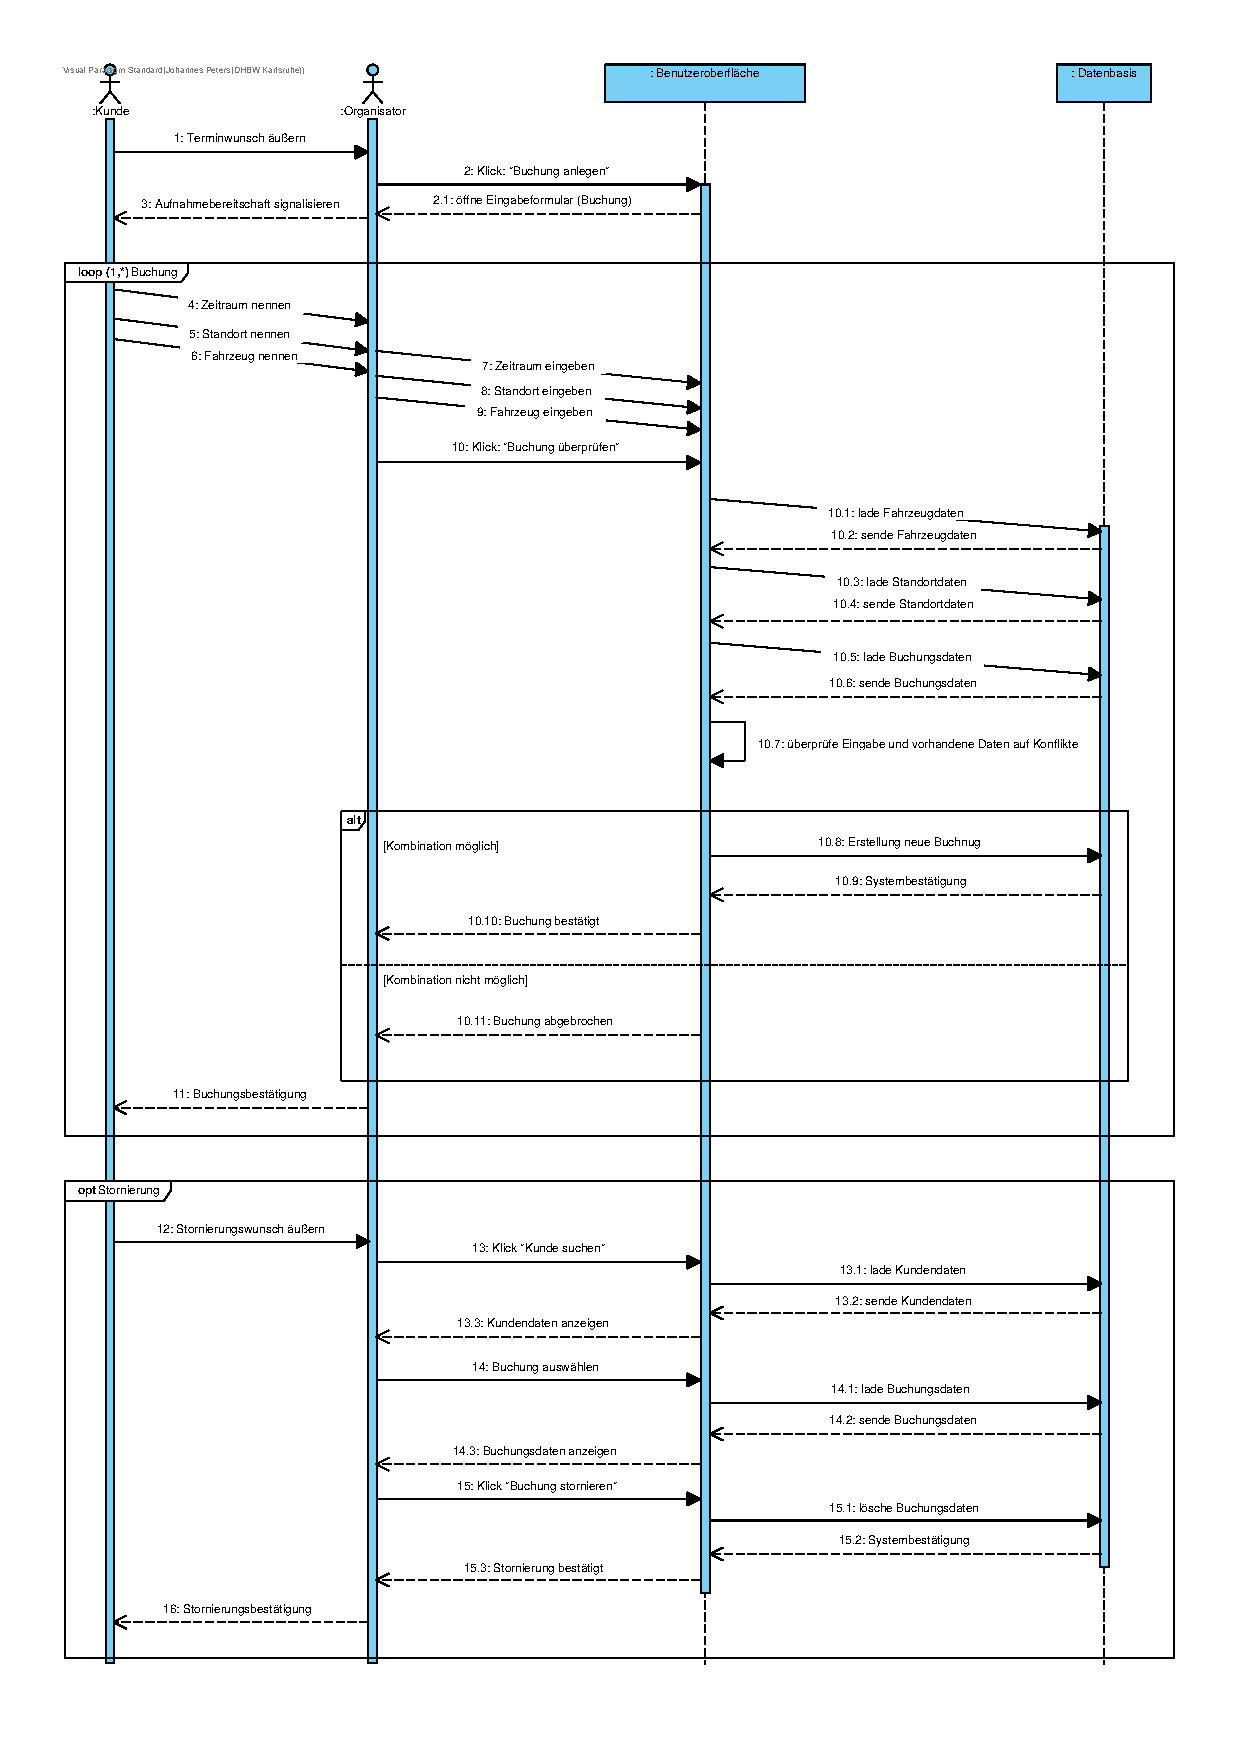
\includegraphics[width=\textwidth, height=\textheight-4cm]{Bilder/Diagramme/SD_Buchungsvorgang_01.pdf}
    \caption{Buchung eines Termins}
    \label{img:buchung01}
\end{figure}

\clearpage

\subsection{Fahrt antreten}

\begin{figure}[!ht]
    \centering
    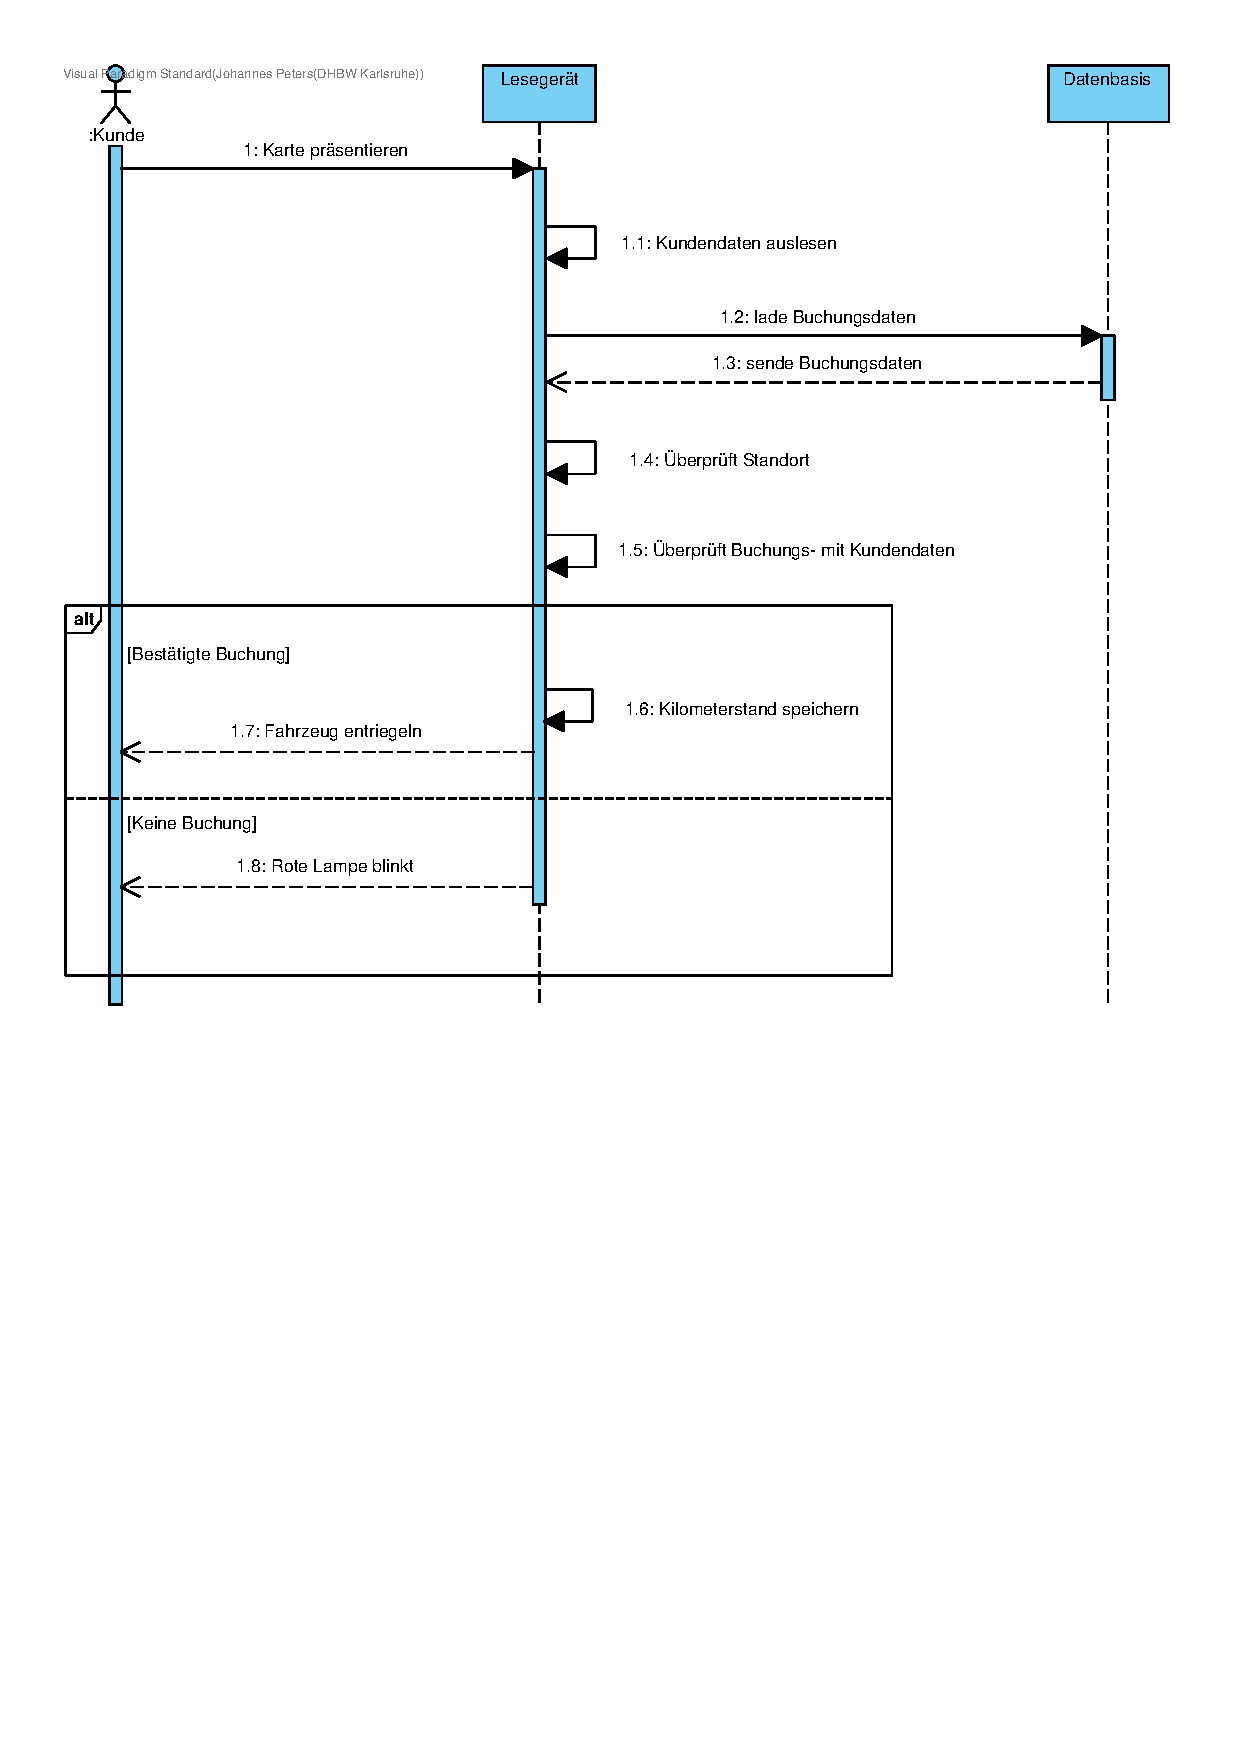
\includegraphics[width=\textwidth, trim = 0cm 13cm 0cm 0cm]{Bilder/Diagramme/SD_Buchungsvorgang_02.pdf}
    \caption{Antritt eines gebuchten Termins}
    \label{img:buchung02}
\end{figure}

\newpage

\subsection{Fahrt beenden}

\begin{figure}[!ht]
    \centering
    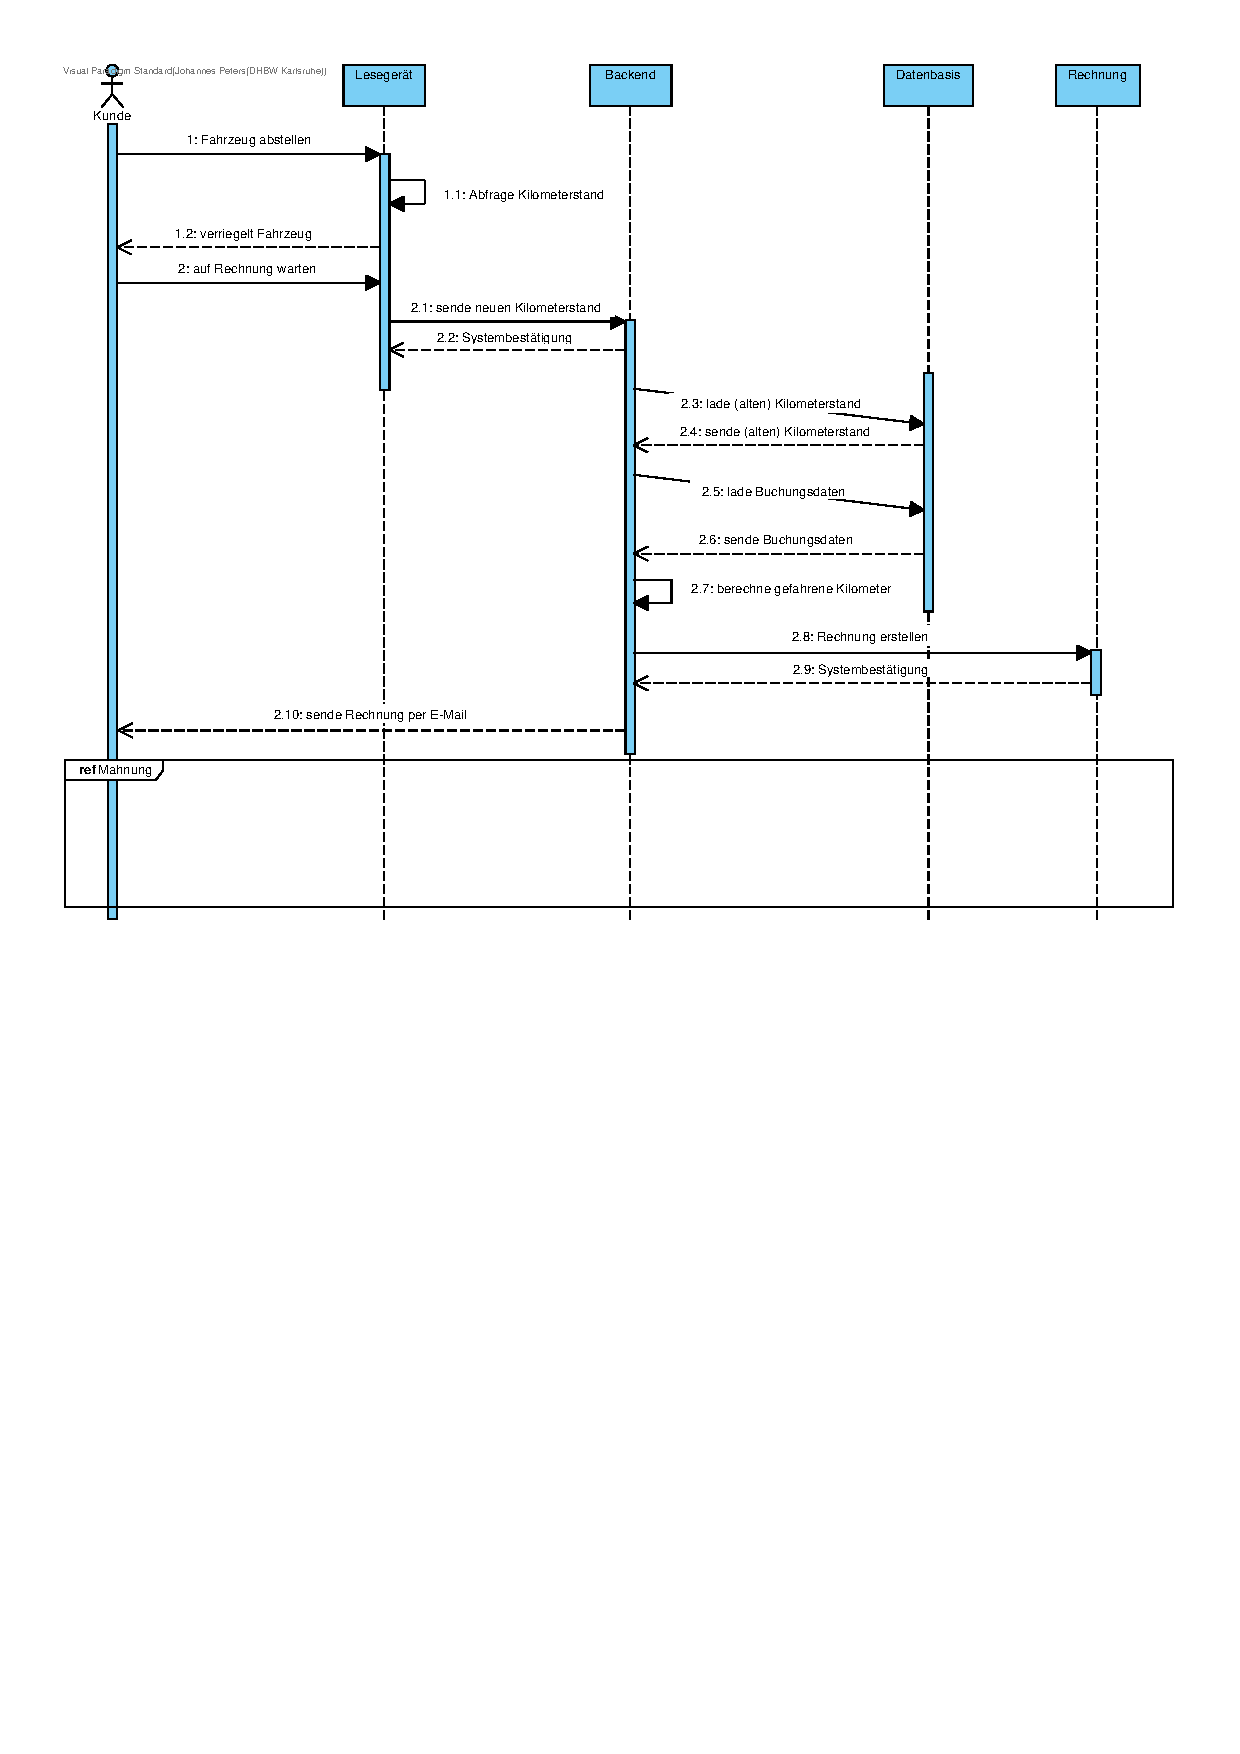
\includegraphics[width=\textwidth, trim = 0cm 14cm 0cm 0cm]{Bilder/Diagramme/SD_Buchungsvorgang_03.pdf}
    \caption{Abschluss eines gebuchten Termins}
    \label{img:buchung03}
\end{figure}

\begin{figure}[!ht]
    \centering
    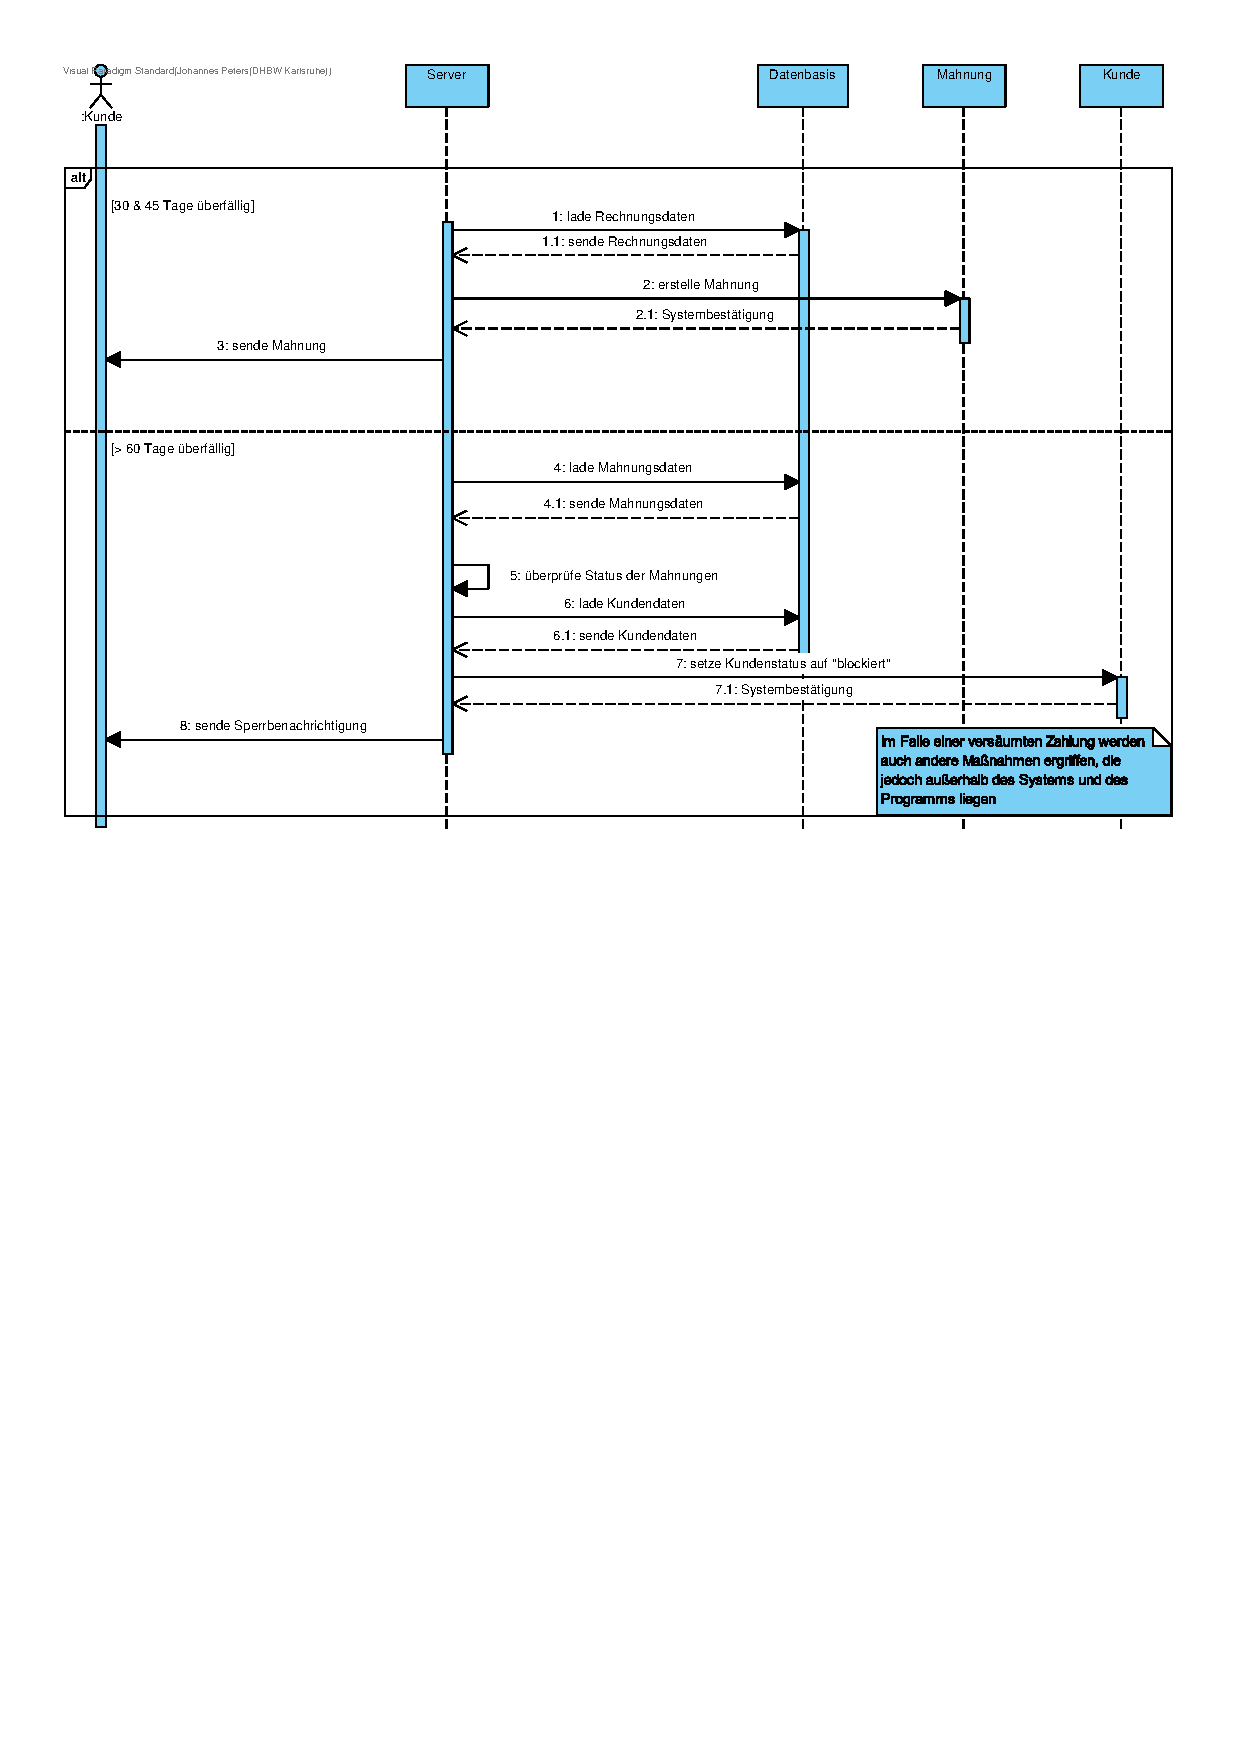
\includegraphics[width=\textwidth, trim = 0cm 16cm 0cm 0cm]{Bilder/Diagramme/SD_Buchungsvorgang_04.pdf}
    \caption{Erstellung der Mahnungen}
    \label{img:buchung04}
\end{figure}
